The goal of this section is to present the overall proof strategy to
establish the semantic preservation property. We use the proof of
Lemma~\nameref{lem:fe-equal-fired}, involved in the proof of
Lemma~\nameref{lem:fe}, to illustrate our demonstration technics. The
proof of Lemma~\nameref{lem:fe-equal-fired} has been one tricky part
of the proof, and therefore, it is worth to be mentioned. Also, it has
led to a bug detection. We give a full account on this bug detection,
and on how we manage to correct it, at the end of the section.

\subsection{Informal presentation of the proof}
\label{sec:informal-fired-proof}

The proof we will detail here pertains to the set of fired
transitions. In an SITPN, the firing process is involved in the
computation of the new marking, the reset orders, and the execution of
functions during the rising edge phase. Therefore, to prove the
semantic preservation property, we must have the equivalence between
the set of fired transitions as defined on the SITPN side and the set
of fired transitions as defined on the \hvhdl{} side. The equivalence
must hold at the beginning of the rising edge phase, i.e, when the set
of fired transitions will be used to compute a new SITPN state.  To
prove the equivalence, we must first look at the definition of the set
of fired transitions on the SITPN and the \hvhdl{} side, and then
think of a way to relate the two definitions.

On the SITPN side, the set of fired transitions receives an
intentional and recursive definition (see Definition~\ref{def:fired})
depending on a given SITPN state. In Lemma~\ref{lem:fe-equal-fired},
we are interested in the definition of the set of fired transitions at
state $s'$, i.e the state at the end of the falling edge phase (which
will also be the state at the beginning of the next rising edge
phase). A transition belongs to the set of fired transitions if it is
\emph{firable} (see Definition~\ref{def:firable}) and sensitized by
the \emph{residual} marking at the considered SITPN state.
Figure~\ref{fig:example-fired-trans} gives the set of fired
transitions, i.e $Fired(s)$, for an example SITPN at a given state
$s$. Here, transitions $t_a$, $t_b$ and $t_c$ are all firable at state
$s$; however, only transition $t_c$ is sensitized by the residual
marking.

\begin{figure}[H]
  \centering
  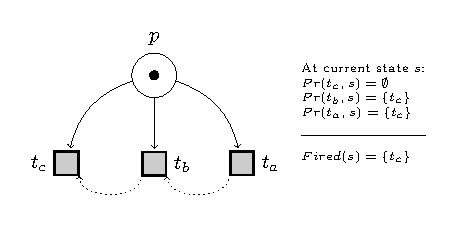
\includegraphics[keepaspectratio,width=.6\textwidth]{Figures/Proof/example-fired-trans}
  \caption[An example of fired transitions set]{The set of fired
    transitions for an example SITPN at a given SITPN state $s$; on
    the right side, the dotted arrows indicates the priority relation
    between the three transitions ($t_c$ is the top-priority
    transition); on the left side, each transition is associated to
    its $Pr$ set which are necessary to compute the residual marking.
  }
  \label{fig:example-fired-trans}
\end{figure}

The computation of the residual marking involves the $Pr$ sets, which
are, for a given transition $t$ and a state $s$, the set of
transitions with a higher firing priority than $t$ which are actually
fired at $s$. This is where the recursive definition of the set of
fired transitions begins. The definition is correct, i.e the recursion
ends, if the priority relation is a strict order over the set of
transitions, and therefore, there are always transitions of
top-priority (e.g, $t_c$ in Figure~\ref{fig:example-fired-trans}). The
condition of the priority relation being a strict order over the set
of transitions is part of the definition of a well-defined SITPN (see
Definition~\ref{def:wd-sitpn}). By definition, top-priority
transitions have an empty $Pr$ set. Indeed, there exist no transition
with a higher firing priority than a top-priority transition. Thus, a
top-priority transition that is firable is also fired. Note that one
can not determine the $Pr$ set of a transition before having
determined the firing status of all the transitions with a higher
firing priority. For instance, in
Figure~\ref{fig:example-fired-trans}, it is impossible to know the
content of $Pr(t_a)$ before having determined if transition $t_b$ is
fired or not. To know if $t_b$ is fired or not, we must determine the
content of $Pr(t_b)$. To do so, we must first determine the firing
status of $t_c$. Even though the definition of the set of fired
transitions is very declarative, this hints at a natural way to
establish an algorithm to build the set of fired transitions at a
given SITPN state.

On the \hvhdl{} side, the set of fired transitions is defined through
the value of the \texttt{fired} port of transition component
instances. The transition design declares an output port of boolean
type with the identifier \texttt{fired}. What we want to prove in
Lemma~\ref{lem:fe-equal-fired} is that, at the end of the falling edge
phase (i.e at state $\sigma'$), the value of the \texttt{fired} port
of a transition component instance reflects the firing status of the
corresponding transition. The \texttt{fired} port is a combinational
signal. This means that its value depends on an equation that is
verified when all signals are stable, i.e at the end of the
stabilization phases happening during the simulation. In the point of
view of the circuit synthesis, this equation reflects the wiring of
the port on the described hardware
circuit. Figure~\ref{fig:fired-port} shows a part of the transition
design architecture describing how the \texttt{fired} port is
connected with to the other internal signals.

\begin{figure}[H]
  \centering
  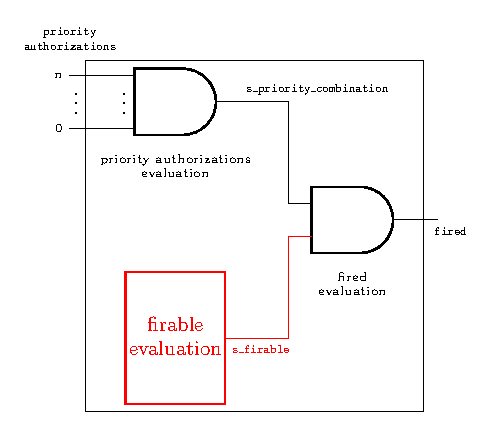
\includegraphics[keepaspectratio,width=.6\textwidth]{Figures/Proof/fired-port}
  \caption[The fired port of the transition design]{Wiring of the
    \texttt{fired} output port in the transition design architecture;
    on the left side is the input interface of the transition design;
    on the right side is the output interface of the transition
    design, with the \texttt{fired} port; in red are the parts of the
    architecture that depend on synchronous logic and in black are the
    parts that are purely combinational.}
  \label{fig:fired-port}
\end{figure}

In Figure~\ref{fig:fired-port}, the labels underneath the and ports
and inside the block denote the names of the processes defined in the
transition design architecture as VHDL code. As a matter of fact,
Figure~\ref{fig:fired-port} is a transcription of the code defining
the transition design architecture. Therefore, by looking at the VHDL
code, we are able to determine the combinational equation associated
to the \texttt{fired} port. Considering a transition component
instance $id_t$ at a given stable state $\sigma$, the \texttt{fired}
port equation is:

\begin{equation}
  \label{eq:fired-port-comb-eq}
  \sigma(id_t)("fired")=\sigma(id_t)("s\_firable")~.~\sigma(id_t)("s\_priority\_combination")
\end{equation}

In Equation~\eqref{eq:fired-port-comb-eq}, $\sigma(id_t)$ denotes the
internal state of the transition component instance $id_t$. From
$\sigma(id_t)$, we have access to the values of the input ports, the
outport ports and the internal signals of the
component. Equation~\eqref{eq:fired-port-comb-eq} states that the
value of the \texttt{fired} port is a simple and expression between
the value of the internal signal \texttt{s\_firable} and
\texttt{s\_priority\_combination}. To differentiate the formulas of
the intuitionistic logic from the expressions of the boolean logic, we
use (``$.$'', ``+'') to denote the \emph{and} and \emph{or} operators
in boolean expressions, and ($\land$,$\lor$) to denote the conjunction
and the disjunction in the intuitionistic formulas.



\subsection{Formal presentation of the proof}
\label{sec:formal-fired-proof}

%%%%%%%%%%%%%%%%%%%%%%%%%%%%%%%%%%%%%%%%%%%%% 
%%%%%%%%%% FALLING EDGE HYPOTHESES %%%%%%%%%%
%%%%%%%%%%%%%%%%%%%%%%%%%%%%%%%%%%%%%%%%%%%%%

\begin{definition}[Falling edge hypotheses]
  \label{def:fe-hyps}
  Given an $sitpn\in{}SITPN$, $d\in{}design$,
  $\gamma\in{}WM(sitpn,d)$,
  $E_c\in\mathbb{N}\rightarrow\mathcal{C}\rightarrow\mathbb{B}$,
  $\Delta\in{}ElDesign(d,\mathcal{D}_\mathcal{H})$,
  $E_p\in(\mathbb{N}\times\{\uparrow,\downarrow\})\rightarrow{}Ins(\Delta)\rightarrow{}value$,
  $\tau\in\mathbb{N}$, $s,s'\in{}S(sitpn)$,
  $\sigma_e,\sigma,\sigma_i,\sigma_\downarrow,\sigma'\in\Sigma(\Delta)$,
  assume that:
  \begin{itemize}
  \item $\lfloor{}sitpn\rfloor_\mathcal{H}=(d,\gamma)$ and
    $\gamma\vdash{}E_p\stackrel{env}{=}E_c$ and
    $\mathcal{D}_\mathcal{H},\emptyset\vdash\mathrm{d}\srarrow{elab}{\fontsize{5}{7}\selectfont}\Delta,\sigma_e$
  \item $\gamma,E_c,\tau\vdash{}s\stackrel{\uparrow}{\approx}\sigma$
  \item $E_c,\tau\vdash{}s\xrightarrow{\downarrow}s'$
  \item $\mathtt{Inject}_\downarrow(\sigma, E_p, \tau, \sigma_i)$
    and
    $\Delta,\sigma_i\vdash\mathrm{d.cs}\xrightarrow{\downarrow}\sigma_{\downarrow}$
    and
    $\Delta,\sigma_{\downarrow}\vdash\mathrm{d.cs}\xrightarrow{\rightsquigarrow}\sigma'$
  \item State $\sigma$ is a stable design state:
    $\mathcal{D}_{\mathcal{H}},\Delta,\sigma\vdash\mathrm{d.cs}\xrightarrow{comb}\sigma$
  \end{itemize}
\end{definition}

\def\fehyps{For all $sitpn$, $d$, $\gamma$, $\Delta$, $\sigma_e$,
  $E_c$, $E_p$, $\tau$, $s$, $s'$, $\sigma$, $\sigma_i$,
  $\sigma_{\downarrow}$, $\sigma'$ that verify the hypotheses of
  Def.~\ref{def:fe-hyps},}

%%%%%%%%%%%%%%%%%%%%%%%%%%%%%%%%%%%%%%%%%%%%%%%%%%%% 
%%%%%%%%%% FALLING EDGE EQUAL FIRED LEMMA %%%%%%%%%%
%%%%%%%%%%%%%%%%%%%%%%%%%%%%%%%%%%%%%%%%%%%%%%%%%%%%

\begin{lemma}[Falling edge equal fired]
  \label{lem:fe-equal-fired}
  \fehyps{} then
  $\forall{}t\in{}T,id_t\in{}Comps(\Delta)~s.t.~\gamma(t)=id_t,$
  $t\in{}Fired(s')\Leftrightarrow\sigma'(id_t)("fired")=\mathtt{true}$.
\end{lemma}

\begin{niproof}
  Given a $t\in{}T$ and an $id_t$ s.t. $\gamma(t)=id_t$, let us show
  \fbox{$t\in{}Fired(s')\Leftrightarrow\sigma'(id_t)("fired")=\mathtt{true}$.}

  The proof is in two parts:
  \begin{enumerate}
  \item Assuming that $t\in{}Fired(s')$, let us show
    \fbox{$\sigma'(id_t)("fired")=\texttt{true}$.}
    
    By definition of $t\in{}Fired(s')$, there exists
    $fset\subseteq{}T$ s.t. $IsFiredSet(s',fset)~\land~t\in{}fset$.
    
    Let us take such an $fset$, and apply
    Lemma~\nameref{lem:fe-equal-fset} to solve the goal.
  \item Assuming that $\sigma'(id_t)("fired")=\mathtt{true}$, let us
    show \fbox{$t\in{}Fired(s')$.}

    By definition of $t\in{}Fired(s')$, let us show that
    \fbox{$\exists{}fset\subseteq{}T$
      s.t. $IsFiredSet(s',fset)~\land~t\in{}fset$}

    Assuming that $sitpn$ is a well-defined $SITPN$ (see Section
    \todo{Add ref. to well-defined SITPN}), we can always find an
    $fset\subseteq{}T$ such that
    $\forall{}s\in{}S(sitpn),~IsFiredSet(s,fset)$ is derivable.  Let
    us take an $fset\subseteq{}T$ s.t. $IsFiredSet(s',fset)$, and use
    it to prove the goal by applying
    Lemma~\nameref{lem:fe-equal-fset}.
    
  \end{enumerate}
\end{niproof}

\begin{lemma}[Falling Edge Equal Not Fired]
  \label{lem:fe-equal-not-fired}
  \fehyps{} then $\forall{}t,id_t~s.t.~\gamma(t)=id_t,$
  $~t\notin{}Fired(s')\Leftrightarrow\sigma'_t("fired")=\mathtt{false}$.
\end{lemma}

\begin{proof}
  Proving the above lemma is trivial by appealing to
  Lemma~\nameref{lem:fe-equal-fired} and by reasoning on
  contrapositives.
\end{proof}

%%%%%%%%%%%%%%%%%%%%%%%%%%%%%%%%%%%%%%%%%%%%%%%%%%%%%%%%
%%%%%%%%%% FALLING EDGE EQUAL FIRED SET LEMMA %%%%%%%%%%
%%%%%%%%%%%%%%%%%%%%%%%%%%%%%%%%%%%%%%%%%%%%%%%%%%%%%%%%


\begin{lemma}[Falling Edge Equal Fired Set]
  \label{lem:fe-equal-fset}
  \fehyps{} then
  $\forall{}t\in{}T,~id_t\in{}Comps(\Delta)~s.t.~\gamma(t)=id_t$,
  $\forall{}fset\subseteq{}T,~s.t.~IsFiredSet(s',fset),~t\in{}fset\Leftrightarrow\sigma'(id_t)("fired")=true$.
\end{lemma}

\begin{niproof}
  Given a $t\in{}T$, and $id_t\in{}Comps(\Delta)$, and a
  $fset\subseteq{}T$ s.t. $IsFiredSet(s',fset)$, let us show
  \fbox{$t\in{}fset\Leftrightarrow\sigma'(id_t)("fired")=true$.}\\

  By definition of $IsFiredSet(s',fset)$, we have
  $IsFiredSetAux(s',\emptyset,T,fset)$.

  Then, we can appeal to Lemma~\nameref{lem:fe-equal-fset-aux} to
  solve the goal, but first we must prove the following \emph{extra
    hypothesis} (i.e, one of the premise of
  Lemma~\nameref{lem:fe-equal-fset-aux}):

  \fbox{\parbox{\lwidth}{$\forall{}t'\in{}T,id_{t'}\in{}Comps(\Delta)$
      s.t. $\gamma(t')=id_{t'},$\\
      $(t'\in{}\emptyset\Rightarrow\sigma'(id_{t'})("fired")=\mathtt{true})$
      $\land$
      $(\sigma'(id_{t'})("fired")=\mathtt{true}\Rightarrow{}t'\in{}\emptyset~\lor~{}t'\in{}T)$.}}\\

  Given a $t'\in{}T$ and an $id_{t'}\in{}Comps(\Delta)$
  s.t. $\gamma(t')=id_{t'}$, there are two points to prove:
  \begin{enumerate}
  \item
    \fbox{$t'\in{}\emptyset\Rightarrow\sigma'(id_{t'})("fired")=\mathtt{true}$}
  \item
    \fbox{$\sigma'(id_{t'})("fired")=\mathtt{true}\Rightarrow{}t'\in{}\emptyset~\lor~{}t'\in{}T$}
  \end{enumerate}

  Let us show these two points:
  \begin{enumerate}
  \item Assuming $t'\in{}\emptyset$, let us show
    \fbox{$\sigma'(id_{t'})("fired")=\mathtt{true}$.}

    \qedbox{$t'\in{}\emptyset$ is a contradiction.}
  \item Assuming $\sigma'(id_{t'})("fired")=\mathtt{true}$, let us
    show \fbox{$t'\in{}\emptyset~\lor~{}t'\in{}T$.}

    By definition, \qedbox{$t'\in{}T$.}
  \end{enumerate}
  
\end{niproof}

%%%%%%%%%%%%%%%%%%%%%%%%%%%%%%%%%%%%%%%%%%%%%%%%%%%%%%%%%%%%
%%%%%%%%%% FALLING EDGE EQUAL FIRED SET AUX LEMMA %%%%%%%%%%
%%%%%%%%%%%%%%%%%%%%%%%%%%%%%%%%%%%%%%%%%%%%%%%%%%%%%%%%%%%%

\begin{lemma}[Falling Edge Equal Fired Set Aux]
  \label{lem:fe-equal-fset-aux}
  \fehyps{} then
  $\forall{}t\in{}T,id_t\in{}Comps(\Delta)~s.t.~\gamma(t)=id_t$,
  $\forall{}fired\subseteq{}T,~T_s\subseteq{}T,~fset\subseteq{}T,$
  assume that:
  \begin{itemize}
  \item $IsFiredSetAux(s',fired,T_s,fset)$
  \item EH (Extra. Hypothesis):\\
    $\forall{}t'\in{}T,~id_{t'}\in{}Comps(\Delta)$
    s.t. $\gamma(t')=id_{t'}$,\\
    $(t'\in{}fired\Rightarrow\sigma'(id_{t'})("fired")=\mathtt{true})$
    $\land$
    $(\sigma'(id_{t'})("fired")=\mathtt{true}\Rightarrow{}t'\in{}fired~\lor~{}t'\in{}T_s)$.
  \end{itemize}
  then
  $t\in{}fset\Leftrightarrow\sigma'(id_t)("fired")=\mathtt{true}$.
\end{lemma}

\begin{niproof}
  Given a $t\in{}T$, an $id_t\in{}Comps(\Delta)$, a
  $fired,T_s,fset\subseteq{}T$, and assuming\\
  $IsFiredSetAux(s',fired,T_s,fset)$ and EH, let us show
  \fbox{$t\in{}fset\Leftrightarrow\sigma'(id_t)("fired")=\mathtt{true}$.}

  Let us reason by induction on $IsFiredSetAux(s',fired,T_s,fset)$.

  \begin{itemize}
  \item \textbf{BASE CASE}:
    \fbox{$t\in{}fired\Leftrightarrow\sigma'(id_t)("fired")=\mathtt{true}$.}

    In that case, $fired=fset$ and $T_s=\emptyset$, EH looks like
    this:

    \parbox{\lwidth}{$\forall{}t'\in{}T,~id_{t'}\in{}Comps(\Delta)$
      s.t. $\gamma(t')=id_{t'}$,\\
      $(t'\in{}fired\Rightarrow\sigma'(id_{t'})("fired")=\mathtt{true})$
      $\land$
      $(\sigma'(id_{t'})("fired")=\mathtt{true}\Rightarrow{}t'\in{}fired~\lor~{}t'\in{}\emptyset)$.}

    From EH, we can deduce
    \qedbox{$t\in{}fired\Leftrightarrow\sigma'(id_t)("fired")=\mathtt{true}$.}
    
  \item \textbf{INDUCTION CASE}:
    \fbox{$t\in{}fset\Leftrightarrow\sigma'(id_t)("fired")=\mathtt{true}$.}

    In that case, we have:
    \begin{itemize}
    \item $IsTopPrioritySet(T_s,tp)$
    \item $ElectFired(s',fired,tp,fired')$
    \item $FiredAux(s',fired',T_s\setminus{}tp,fset)$
    \end{itemize}

    \begin{ih}
      $\big(\forall{}t'\in{}T,id_{t'}\in{}Comps(\Delta)~s.t.~\gamma(t')=id_{t'},$\\
      $(t'\in{}fired'\Rightarrow\sigma'(id_{t'})("fired")=\mathtt{true})$
      $\land(\sigma'(id_{t'})("fired")=\mathtt{true}\Rightarrow{}t'\in{}fired'~\lor~{}t'\in{}T_s\setminus{}tp)\big)\Rightarrow$\\
      $t\in{}fset\Leftrightarrow\sigma'_t("fired")=true$.
    \end{ih}
    
    Applying the induction hypothesis, then, the new goal is:
    \begin{frameb}
      $\forall{}t'\in{}T,id_{t'}\in{}Comps(\Delta)~s.t.~\gamma(t')=id_{t'},$\\
      $(t'\in{}fired'\Rightarrow\sigma'(id_{t'})("fired")=\mathtt{true})$\\
      $\land(\sigma'(id_{t'})("fired")=\mathtt{true}\Rightarrow{}t'\in{}fired'~\lor~{}t'\in{}T_s\setminus{}tp)$
    \end{frameb}
    
    Apply Lemma~\nameref{lem:elect-fired-equal-fired} to solve the goal.
    
  \end{itemize}
  
\end{niproof}

%%%%%%%%%%%%%%%%%%%%%%%%%%%%%%%%%%%%%%%%%%%%%
%%%%%%%%%% ELECT FIRED EQUAL FIRED %%%%%%%%%%
%%%%%%%%%%%%%%%%%%%%%%%%%%%%%%%%%%%%%%%%%%%%%

\begin{lemma}[Elect Fired Equal Fired]
  \label{lem:elect-fired-equal-fired}
  \fehyps{} then
  $\forall{}fired,fired',T_s,tp,~fset\subseteq{}T,$
  assume that:
  \begin{itemize}
  \item $IsTopPrioritySet(T_s,tp)$
  \item $ElectFired(s',fired,tp,fired')$
  \item $FiredAux(s',fired',T_s\setminus{}tp,fset)$
  \item EH (Extra. Hypothesis):\\
    $\forall{}t'\in{}T,id_{t'}\in{}Comps(\Delta)~s.t.~\gamma(t')=id_{t'}$,\\
    $(t'\in{}fired\Rightarrow\sigma'(id_{t'})("fired")=\mathtt{true})$
    $\land$
    $(\sigma'(id_{t'})("fired")=\mathtt{true}\Rightarrow{}t'\in{}fired~\lor~{}t'\in{}T_s)$
  \end{itemize}
  then $\forall{}t\in{}T,id_t\in{}Comps(\Delta)$
  s.t. $\gamma(t)=id_t$,\\
  $\big(t\in{}fired'\Rightarrow\sigma'(id_t)("fired")=\mathtt{true}\big)$
  $\land\big(\sigma'(id_t)("fired")=\mathtt{true}\Rightarrow{}t\in{}fired'\lor{}t\in{}T_s\setminus{}tp\big)$.
\end{lemma}

\begin{niproof}
  Given a $t\in{}T$ and an $id_t\in{}Comps(\Delta)$
  s.t. $\gamma(t)=id_t$, let us show\\
  \fbox{$\big(t\in{}fired'\Rightarrow\sigma'(id_t)("fired")=\mathtt{true}\big)$
    $\land\big(\sigma'(id_t)("fired")=\mathtt{true}\Rightarrow{}t\in{}fired'\lor{}t\in{}T_s\setminus{}tp\big)$.}\\
  
  Let us reason by induction on $ElectFired(s',fired,tp,fired')$;
  there are three cases:

  \begin{enumerate}
  \item \textbf{BASE CASE}: $tp=\emptyset$ and $fired=fired'$.
  \item \textbf{INDUCTIVE CASE}: $tp=\{t_0\}\cup{}tp_0$ and $t_0$ is
    elected to be fired.
  \item \textbf{INDUCTIVE CASE}: $tp=\{t_0\}\cup{}tp_0$ and $t_0$ is
    not elected to be fired.
  \end{enumerate}

  Let us prove the goal in these three contexts:

  \begin{enumerate}
  \item \textbf{BASE CASE}:
    
    \fbox{\parbox{\lwidth}{$\big(t\in{}fired\Rightarrow\sigma'(id_t)("fired")=\mathtt{true}\big)$
        $\land\big(\sigma'(id_t)("fired")=\mathtt{true}\Rightarrow{}t\in{}fired\lor{}t\in{}T_s\big)$.}}
    
    \qedbox{Apply EH to solve the goal.}
    
  \item \textbf{INDUCTIVE CASE}: $tp=\{t_0\}\cup{}tp_0$ and $t_0$ is
    elected to be fired.

    In that case, we have:
    \begin{itemize}
    \item
      $IsTopPrioritySet(T_s,\{t_0\}\cup{}tp_0)$
    \item $ElectFired(s',fired\cup\{t_0\},tp_0,fired')$
    \item
      $IsFiredSetAux(s',fired',T_s\setminus\{t_0\}\cup{}tp_0,fset)$
    \item $t_0\in{}Firable(s')$
    \item
      $t_0\in{}Sens(s'.M-\sum\limits_{t_i\in{}Pr(t,fired)}pre(t_i))$
      where $Pr(t,fired)=\{t'~\vert~t'\succ{}t\land{}t'\in{}fired\}$
    \item EH: $\forall{}t'\in{}T,~id_{t'}\in{}Comps(\Delta)$
      s.t. $\gamma(t')=id_{t'}$,\\
      $(t'\in{}fired\Rightarrow\sigma'(id_{t'})("f")=\mathtt{true})$
      $\land$
      $(\sigma'(id_{t'})("f")=\mathtt{true}\Rightarrow{}t'\in{}fired~\lor~{}t'\in{}T_s)$
    \end{itemize}

    \begin{ih}
      $\forall{}T'_s\subseteq{}T,~$\\
      $IsTopPrioritySet(T'_s,tp_0)\Rightarrow$\\
      $IsFiredSetAux(s',fired',T'_s\setminus{}tp_0,fset)\Rightarrow$\\
      $\big(\forall{}t'\in{}T,id_{t'}\in{}Comps(\Delta)$ s.t. $\gamma(t')=id_{t'}$,\\
      $(t'\in{}fired\cup\{t_0\}\Rightarrow\sigma'_{t'}("f")=\mathtt{true})$
      $\land$
      $(\sigma'(id_{t'})("f")=\mathtt{true}\Rightarrow{}t'\in{}fired\cup\{t_0\}~\lor~{}t'\in{}T'_s)\big)\Rightarrow$\\
      $\forall{}t\in{}T,~id_t\in{}Comps(\Delta)$ s.t. $\gamma(t)=id_t$,\\
      $~\big(t\in{}fired'\Rightarrow\sigma'(id_t)("f")=\mathtt{true}\big)$
      $\land$
      $\big(\sigma'(id_t)("f")=\mathtt{true}\Rightarrow{}t\in{}fired'\lor{}t\in{}T'_s\setminus{}tp_0\big)$
    \end{ih}
    
    \begin{frameb}
      $\forall{}t\in{}T,~id_t\in{}Comps(\Delta)$
      s.t. $\gamma(t)=id_t$,\\
      $~\big(t\in{}fired'\Rightarrow\sigma'_t("f")=\mathtt{true}\big)$
      $\land$
      $\big(\sigma'_t("f")=\mathtt{true}\Rightarrow{}t\in{}fired'\lor{}t\in{}T_s\setminus{}\{t_0\}\cup{}tp_0\big)$
    \end{frameb}
    
    To solve the goal, we can apply the induction hypothesis with
    $T'_s=T_s\setminus\{t_0\}$; then, there are three points to prove:
    \begin{enumerate}
    \item
      \fbox{$IsTopPrioritySet(T_s\setminus\{t_0\},tp_0)$}
    \item
      \fbox{$IsFiredSetAux(s',fired',(T_s\setminus\{t_0\})\setminus{}tp_0,fset)$}
    \item \fbox{\parbox{\lwidth}{$\forall{}t'\in{}T,id_{t'}\in{}Comps(\Delta)$ s.t. $\gamma(t')=id_{t'}$,\\
          $(t'\in{}fired\cup\{t_0\}\Rightarrow\sigma'_{t'}("f")=\mathtt{true})$
          $\land$
          $(\sigma'(id_{t'})("f")=\mathtt{true}\Rightarrow{}t'\in{}fired\cup\{t_0\}~\lor~{}t'\in{}T_s\setminus\{t_0\})$}}
    \end{enumerate}

    Let us prove these three points:
    \begin{enumerate}
    \item
      \fbox{$IsTopPrioritySet(T_s\setminus\{t_0\},tp_0)$}
      \begin{todobox}
        Not provable yet.
      \end{todobox}
    \item
      \fbox{$IsFiredSetAux(s',fired',(T_s\setminus\{t_0\})\setminus{}tp_0,fset)$}.
      
      We know that
      $(T_s\setminus\{t_0\})\setminus{}tp_0=T_s\setminus{}(\{t_0\}\cup{}tp_0)$,
      and thus\\
      \qedbox{$IsFiredSetAux(s',fired',T_s\setminus{}(\{t_0\}\cup{}tp_0),fset)$
        is an assumption.}
      
    \item \fbox{\parbox{\lwidth}{$\forall{}t'\in{}T,id_{t'}\in{}Comps(\Delta)$ s.t. $\gamma(t')=id_{t'}$,\\
          $(t'\in{}fired\cup\{t_0\}\Rightarrow\sigma'(id_{t'})("f")=\mathtt{true})$
          $\land$
          $(\sigma'(id_{t'})("f")=\mathtt{true}\Rightarrow{}t'\in{}fired\cup\{t_0\}~\lor~{}t'\in{}T_s\setminus\{t_0\})$}}\\

      Given a $t'\in{}T$ and an $id_{t'}\in{}Comps(\Delta)$
      s.t. $\gamma(t')=id_{t'}$, let us show\\
      \fbox{\parbox{\lwidth}{$(t'\in{}fired\cup\{t_0\}\Rightarrow\sigma'(id_{t'})("f")=\mathtt{true})$\\
          $\land$
          $(\sigma'(id_{t'})("f")=\mathtt{true}\Rightarrow{}t'\in{}fired\cup\{t_0\}~\lor~{}t'\in{}T_s\setminus\{t_0\})$.}}
      
      The proof is in two parts.
      
      \begin{enumerate}
      \item Assuming that $t'\in{}fired\cup\{t_0\}$, let us show
        \fbox{$\sigma'(id_{t'})("f")=\mathtt{true}$.}

        Case analysis on $t'\in{}fired\cup\{t_0\}$; there are two cases:
        \begin{itemize}
        \item $t'\in{}fired$
        \item $t'=t_0$
        \end{itemize}

        Let us prove the goal in these two contexts.
        
        \begin{itemize}
        \item \textbf{CASE} $t'\in{}fired$: Thanks to EH, we can
          deduce \qedbox{$\sigma'_{t'}("f")=\mathtt{true}$.}
          
        \item \textbf{CASE} $t'=t_0$:
          
          By definition of $id_{t'}$, there exist a $gm_{t'}$,
          $ipm_{t'}$, $opm_{t'}$ s.t.
          $\mathtt{comp}(id_{t'},"transition",$ $gm_{t'},$ $ipm_{t'}$,
          $opm_{t'})\in{}d.cs$.

          By property of the stabilize relation and
          $\mathtt{comp}(id_{t'},"transition",$ $gm_{t'},$ $ipm_{t'}$,
          $opm_{t'})\in{}d.cs$:
          \begin{equation}
            \label{eq:frd-eq-frd}
            \sigma(id_{t'})("f")=\sigma(id_{t'})("sfa")~.~\sigma(id_{t'})("spc")
          \end{equation}

          Rewriting the goal with \eqref{eq:frd-eq-frd}:
          \fbox{$\sigma(id_{t'})("sfa")~.~\sigma(id_{t'})("spc")=\mathtt{true}$.}
          
          Then, we can show that: 
          \begin{itemize}
          \item $\sigma(id_{t'})("sfa")=\mathtt{true}$ by applying
            Lemma~\nameref{lem:fe-equal-firable}
          \item $\sigma(id_{t'})("spc")=\mathtt{true}$ by applying
            Lemma~\nameref{lem:stab-compute-pcomb}.
          \end{itemize}
        \end{itemize}
        
      \item Assuming that $\sigma'(id_{t'})("f")=\mathtt{true}$, let
        us show
        \fbox{$t'\in{}fired\cup\{t_0\}~\lor~{}t'\in{}T_s\setminus{}\{t_0\}$.}

        From $\sigma'(id_{t'})("f")=\mathtt{true}$ and EH, we can
        deduce that $t'\in{}fired\lor{}t'\in{}T_s$.

        Case analysis on $t'\in{}fired\lor{}t'\in{}T_s$.
        
        \begin{itemize}
        \item \textbf{CASE} $t'\in{}fired$: then, it is trivial to
          show \qedbox{$t'\in{}fired\cup\{t_0\}$.}
        \item \textbf{CASE} $t'\in{}T_s$: We know that $t_0\in{}T_s$.
          Therefore, either \qedbox{$t'\in{}T_s\setminus{}\{t_0\}$},
          or $t'=t_0$, and then, \qedbox{$t'\in{}fired\cup\{t_0\}$.}
        \end{itemize}
      \end{enumerate}
    \end{enumerate}
  \end{enumerate}

  \begin{enumerate}[resume]
  \item \textbf{INDUCTIVE CASE}: $tp=\{t_0\}\cup{}tp_0$ and $t_0$ is
    not elected to be fired.
    \begin{itemize}
    \item $IsTopPrioritySet(T_s,\{t_0\}\cup{}tp_0)$
    \item $ElectFired(s',fired,tp_0,fired')$
    \item $IsFiredSetAux(s',fired',T_s\setminus\{t_0\}\cup{}tp_0,fset)$
    \item $\neg\big(t_0\in{}Firable(s')\land{}t_0\in{}Sens(s'.M-\sum\limits_{t_i\in{}Pr(t,fired)}pre(t_i))\big)$
    \item EH:\\
      $\forall{}t'\in{}T,id_{t'}\in{}Comps(\Delta)$ s.t. $\gamma(t')=id_{t'}$,\\
      $(t'\in{}fired\Rightarrow\sigma'(id_{t'})("f")=\mathtt{true})$
      $\land$
      $(\sigma'(id_{t'})("f")=\mathtt{true}\Rightarrow{}t'\in{}fired~\lor~{}t'\in{}T_s)$
    \end{itemize}

    \begin{ih}
      $\forall{}T'_s\subseteq{}T,~$\\
      $IsTopPrioritySet(T'_s,tp_0)\Rightarrow$\\
      $IsFiredSetAux(s',fired',T'_s\setminus{}tp_0,fset)\Rightarrow$\\
      $\big(\forall{}t'\in{}T,id_{t'}\in{}Comps(\Delta)$
      s.t. $\gamma(t')=id_{t'},$\\
      $(t'\in{}fired\Rightarrow\sigma'(id_{t'})("f")=\mathtt{true})$
      $\land$
      $(\sigma'(id_{t'})("f")=\mathtt{true}\Rightarrow{}t'\in{}fired~\lor~{}t'\in{}T'_s)\big)\Rightarrow$\\
      $\forall{}t\in{}T,id_t\in{}Comps(\Delta)$ s.t. $\gamma(t)=id_t$,\\
      $~\big(t\in{}fired'\Rightarrow\sigma'(id_t)("f")=\mathtt{true}\big)$
      $\land$
      $\big(\sigma'(id_t)("f")=\mathtt{true}\Rightarrow{}t\in{}fired'\lor{}t\in{}T'_s\setminus{}tp_0\big)$
    \end{ih}
    
    \fbox{\parbox{\lwidth}{$\forall{}t\in{}T,id_t\in{}Comps(\Delta)$ s.t. $\gamma(t)=id_t$,\\
        $~\big(t\in{}fired'\Rightarrow\sigma'(id_t)("f")=\mathtt{true}\big)$
        $\land$
        $\big(\sigma'(id_t)("f")=\mathtt{true}\Rightarrow{}t\in{}fired'\lor{}t\in{}T_s\setminus{}\{t_0\}\cup{}tp_0\big)$.}}
    
    Then, we can apply the induction hypothesis with
    $T'_s=T_s\setminus\{t_0\}$, then, there are three points to prove:

    \begin{enumerate}
    \item
      \fbox{$IsTopPrioritySet(T_s\setminus\{t_0\},tp_0)$}
    \item
      \fbox{$IsFiredSetAux(s',fired',(T_s\setminus\{t_0\})\setminus{}tp_0,fset)$}
    \item \fbox{\parbox{\lwidth}{$\forall{}t'\in{}T,id_{t'}\in{}Comps(\Delta)$
          s.t. $\gamma(t')=id_{t'}$,\\
          $(t'\in{}fired\Rightarrow\sigma'(id_{t'})("f")=\mathtt{true})$
          $\land$
          $(\sigma'(id_{t'})("f")=\mathtt{true}\Rightarrow{}t'\in{}fired~\lor~{}t'\in{}T_s\setminus\{t_0\})$}}
    \end{enumerate}

    Let us prove these three points:

    \begin{enumerate}
    \item \fbox{$IsTopPrioritySet(T_s\setminus\{t_0\},tp_0)$}
      \begin{todobox}
        Not provable yet.
      \end{todobox}
    \item
      \fbox{$IsFiredSetAux(s',fired',(T_s\setminus\{t_0\})\setminus{}tp_0,fset)$}

      We know that
      $(T_s\setminus\{t_0\})\setminus{}tp_0=T_s\setminus{}(\{t_0\}\cup{}tp_0)$,
      and thus\\
      \qedbox{$IsFiredSetAux(s',fired',T_s\setminus{}(\{t_0\}\cup{}tp_0),fset)$
        is an assumption.}
      
    \item
      \fbox{\parbox{\lwidth}{$\forall{}t'\in{}T,id_{t'}\in{}Comps(\Delta)$
          s.t. $\gamma(t')=id_{t'}$,\\
          $(t'\in{}fired\Rightarrow\sigma'(id_{t'})("f")=\mathtt{true})$
          $\land$
          $(\sigma'(id_{t'})("f")=\mathtt{true}\Rightarrow{}t'\in{}fired~\lor~{}t'\in{}T_s\setminus\{t_0\})$}}

      Given a $t'\in{}T$ and an $id_{t'}\in{}Comps(\Delta)$
      s.t. $\gamma(t')=id_{t'}$, let us show

      \begin{frameb}
        $(t'\in{}fired\Rightarrow\sigma'(id_{t'})("f")=\mathtt{true})$
        $\land$
        $(\sigma'(id_{t'})("f")=\mathtt{true}\Rightarrow{}t'\in{}fired~\lor~{}t'\in{}T_s\setminus\{t_0\})$
      \end{frameb}

      The proof is in two parts:
      
      \begin{enumerate}
      \item Assuming that $t'\in{}fired$, let us show
        \fbox{$\sigma'(id_{t'})("f")=\mathtt{true}$.}

        From $t'\in{}fired$ and EH,
        \qedbox{$\sigma'(id_{t'})("f")=\mathtt{true}$.}
        
      \item Assuming that $\sigma'(id_{t'})("f")=\mathtt{true}$, let
        us show
        \fbox{$t'\in{}fired~\lor~{}t'\in{}T_s\setminus{}\{t_0\}$.}

        Thanks to $\sigma'(id_{t'})("f")=\mathtt{true}$ and EH, we
        know that: $t'\in{}fired\lor{}t'\in{}T_s$.

        Case analysis on $t'\in{}fired\lor{}t'\in{}T_s$; there are two
        cases:
        \begin{itemize}
        \item \textbf{CASE} \qedbox{$t'\in{}fired$.}
        \item \textbf{CASE} $t'\in{}T_s$:

          From $IsTopPrioritySet(T_s,\{t_0\}\cup{}tp_0)$, we can
          deduce that $t_0\in{}T_s$. Therefore, either
          \qedbox{$t'\in{}T_s\setminus{}\{t_0\}$} or $t'=t_0$.

          In the case where $t'=t_0$, we need to show a contradiction by proving\\
          $t'\in{}Firable(s')$ and
          $t'\in{}Sens(s'.M-\sum\limits_{t_i\in{}Pr(t,fired)}pre(t_i))$
          based on $\sigma'(id_{t'})("f")=\mathtt{true}$.

          By definition of $id_{t'}$, there exist a $gm_{t'}$,
          $ipm_{t'}$, $opm_{t'}$ s.t.
          $\mathtt{comp}(id_{t'},"transition",$ $gm_{t'},$ $ipm_{t'}$,
          $opm_{t'})\in{}d.cs$.

          By property of the stabilize relation and
          $\mathtt{comp}(id_{t'},$ $"transition",$ $gm_{t'},$
          $ipm_{t'}$, $opm_{t'})\in{}d.cs$:
          \begin{equation}
            \label{eq:frd-eq-frd-true}
            \sigma(id_{t'})("f")=\sigma(id_{t'})("sfa")~.~\sigma(id_{t'})("spc")=\mathtt{true}
          \end{equation}

          From $\sigma(id_{t'})("sfa")=\mathtt{true}$, and appealing
          to Lemma~\nameref{lem:fe-equal-firable}, we can deduce
          $t'\in{}Firable(s')$.

          From $\sigma(id_{t'})("spc")=\mathtt{true}$, and appealing
          to Lemma~\nameref{lem:stab-compute-pcomb}, we can deduce
          $t'\in{}Sens(s'.M-\sum\limits_{t_i\in{}Pr(t,fired)}$ $pre(t_i))$.

          Then, as $t'=t_0$,
          $\neg\big(t_0\in{}Firable(s')\land{}t_0\in{}Sens(s'.M-\sum\limits_{t_i\in{}Pr(t,fired)}pre(t_i))\big)$
          is a \qedbox{contradiction.}
        \end{itemize}
      \end{enumerate}      
    \end{enumerate}
  \end{enumerate}
  
\end{niproof}

%%%%%%%%%%%%%%%%%%%%%%%%%%%%%%%%%%%%%%%%%%%%%%%%%%%%%%%%%%%%%%%%%%%%%%%%%%%%%%%
%%%%%%%%%% STABILIZE COMPUTE PRIORITY COMBINATION AFTER FALLING EDGE %%%%%%%%%%
%%%%%%%%%%%%%%%%%%%%%%%%%%%%%%%%%%%%%%%%%%%%%%%%%%%%%%%%%%%%%%%%%%%%%%%%%%%%%%%

\begin{lemma}[Stabilize Compute Priority Combination After Falling Edge]
  \label{lem:stab-compute-pcomb}
  \fehyps{} then
  $\forall{}t\in{}T,id_t\in{}Comps(\Delta)$ s.t. $\gamma(t)=id_t$,\\
  $\forall{}fired,fired',~T_s,~tp,~fset\subseteq{}T$ assume that:
  \begin{itemize}
  \item $IsTopPrioritySet(T_s,\{t\}\cup{}tp)$
  \item $ElectFired(s',fired,tp,fired')$
  \item $FiredAux(s',fired',T_s\setminus{}\{t\}\cup{}tp,fset)$
  \item EH: $\forall{}t'\in{}T,id_{t'}\in{}Comps(\Delta)$
    s.t. $\gamma(t')=id_{t'}$,\\
    $(t'\in{}fired\Rightarrow\sigma'(id_{t'})("f")=\mathtt{true})$
    $\land$
    $(\sigma'(id_{t'})("f")=\mathtt{true}\Rightarrow{}t'\in{}fired~\lor~{}t'\in{}T_s)$.
  \item $t\in{}Firable(s')$
  \end{itemize}
  then
  $t\in{}Sens(s'.M-\sum\limits_{t_i\in{}Pr(t,fired)}pre(t_i))\Leftrightarrow\sigma'(id_t)("spc")=\mathtt{true}$
\end{lemma}

\begin{niproof}

  Given a $t\in{}T$ and an $id_t\in{}Comps(\Delta)$
  s.t. $\gamma(t)=id_t$, a $fired$, $fired'$, $T_s$, $tp$,
  $fset\subseteq{}T$ and assuming all the above hypotheses, let us
  show\\
  \fbox{$t\in{}Sens(s'.M-\sum\limits_{t_i\in{}Pr(t,fired)}pre(t_i))\Leftrightarrow\sigma'(id_t)("spc")=\mathtt{true}$.}\\

  \exT{}
  
  By property of the stabilize relation and \InCsCompT:  
  \begin{equation}
    \sigma'(id_t)("spc")=\prod\limits_{i=0}^{\Delta(id_t)("ian")-1}\sigma'(id_t)("pauths")[i]\label{eq:frd-eq-spc-prod-pauths}
  \end{equation}

  Rewriting the goal with \eqref{eq:frd-eq-spc-prod-pauths}:
  
  \fbox{$t\in{}Sens(s'.M-\sum\limits_{t_i\in{}Pr(t,fired)}pre(t_i))\Leftrightarrow\prod\limits_{i=0}^{\Delta(id_t)("ian")-1}\sigma'(id_t)("pauths")[i]=\mathtt{true}$.}\\
  
  Then, the proof is in two parts:
  \begin{enumerate}
  \item
    $t\in{}Sens(s'.M-\sum\limits_{t_i\in{}Pr(t,fired)}pre(t_i))\Rightarrow\prod\limits_{i=0}^{\Delta(id_t)("ian")-1}\sigma'(id_t)("pauths")[i]=\mathtt{true}$
  \item
    $\prod\limits_{i=0}^{\Delta(id_t)("ian")-1}\sigma'(id_t)("pauths")[i]=\mathtt{true}\Rightarrow{}t\in{}Sens(s'.M-\sum\limits_{t_i\in{}Pr(t,fired)}pre(t_i))$
  \end{enumerate}

  Let us prove both sides of the equivalence:
  \begin{enumerate}
  \item\label{item:stab-comp-spc-fst-case}
    Assuming that
    $t\in{}Sens(s'.M-\sum\limits_{t_i\in{}Pr(t,fired)}pre(t_i))$, let
    us
    show\\
    \fbox{$\prod\limits_{i=0}^{\Delta(id_t)("ian")-1}\sigma'(id_t)("pauths")[i]=\mathtt{true}$.}

    Let us perform case analysis on $input(t)$; there are 2 cases:
    \begin{itemize}
    \item \textbf{CASE} $input(t)=\emptyset$:

      By construction,
      ${<}\mathtt{input\_arcs\_number\Rightarrow}{}1{>}\in{}gm_t$ and\\
      ${<}\mathtt{priority\_authorizations(0)\Rightarrow{}true}{>}\in{}ipm_t$.

      By property of the elaboration relation, we have
      $\Delta(id_t)("ian")=1$, and by property of the stabilize
      relation, we have $\sigma'(id_t)("pauths")[0]=\mathtt{true}$.
      
      Rewriting the goal with $\Delta(id_t)("ian")=1$ and
      $\sigma'(id_t)("pauths")[0]=\mathtt{true}$, and simplifying the
      goal: \qedbox{tautology.}
      
    \item \textbf{CASE} $input(t)\neq{}\emptyset$:

      Then, let us show an equivalent goal:\\
      \fbox{$\forall{}i\in[0,\Delta(id_t)("ian")-1],~\sigma'(id_t)("pauths")[i]=\mathtt{true}$.}

      Given an $i\in{}[0,\Delta(id_t)("ian")-1]$, let us show
      \fbox{$\sigma'(id_t)("pauths")[i]=\mathtt{true}$.}

      By construction,
      ${<}\mathtt{input\_arcs\_number\Rightarrow}{}\vert{}input(t)\vert{>}\in{}gm_t$.

      By property of the elaboration relation, we have
      $\Delta(id_t)("ian")=\vert{}input(t)\vert$. Then, we can deduce
      $i\in{}[0,\vert{}input(t)\vert-1]$.
      
      By construction, for all $i\in{}[0,\vert{}input(t)\vert-1]$,
      there exist a $p\in{}input(t)$ and an $id_p\in{}Comps(\Delta)$
      s.t. $\gamma(p)=id_p$, there exist a $gm_p$, $ipm_p$, $opm_p$
      s.t. $\mathtt{comp}(id_p,$ $"place",$ $gm_p,$ $ipm_p,$
      $opm_p)\in{}d.cs$, and there exist a
      $j\in{}[0,\vert{}output(p)\vert]$ and an
      $id_{ji}\in{}Sigs(\Delta)$ s.t.\\
      ${<}\mathtt{input\_arcs\_valid(i)\Rightarrow{}id_{ji}}{>}\in{}ipm_t$
      and
      ${<}\mathtt{output\_arcs\_valid(j)\Rightarrow{}id_{ji}}{>}\in{}opm_t$.
      Let us take such a $p\in{}input(t)$, $id_p\in{}Comps(\Delta)$,
      $gm_p$, $ipm_p$, $opm_p$, $j\in{}[0,$ $\vert{}output(p)\vert]$ and
      $id_{ji}\in{}Sigs(\Delta)$.

      Now, let us perform case analysis on the nature of the arc
      connecting $p$ and $t$; there are 2 cases:
      
      \begin{itemize}
      \item \textbf{CASE} $pre(p,t)=(\omega,\mathtt{test})$ or
        $pre(p,t)=(\omega,\mathtt{inhib})$:

        By construction,
        ${<}\mathtt{priority\_authorizations(i)\Rightarrow{}true}{>}\in{}ipm_t$,
        and by property of the stabilize relation:
        \qedbox{$\sigma'(id_t)("pauths")[i]=\mathtt{true}$.}

      \item \textbf{CASE} $pre(p,t)=(\omega,\mathtt{basic})$:

        Let us define
        $output_c(p)=\{t\in{}T~\vert~\exists{}\omega,~pre(p,t)=(\omega,\mathtt{basic})\}$,
        the set of output transitions of $p$ that are in
        conflict. Then, there are two cases, one for each way to solve
        the conflicts between the output transitions of $p$:

        \begin{itemize}
        \item \textbf{CASE} For all pair of transitions in
          $output_c(p)$, all conflicts are solved by mutual exclusion:

          By construction,
          ${<}\mathtt{priority\_authorizations(i)\Rightarrow{}true}{>}\in{}ipm_t$,
          and by property of the stabilize relation:
          \qedbox{$\sigma'(id_t)("pauths")[i]=\mathtt{true}$.}
        \item \textbf{CASE} The priority relation is a strict total
          order over the set $output_c(p)$:

          By construction, there exists an $id'_{ji}\in{}Sigs(\Delta)$
          s.t.\\
          ${<}\mathtt{priority\_authorizations(i)\Rightarrow{}id'_{ji}}{>}\in{}ipm_t$
          and\\
          ${<}\mathtt{priority\_authorizations(j)\Rightarrow{}id'_{ji}}{>}\in{}opm_p$.

          By property of the stabilize relation, \InCsCompT{} and
          \InCsCompP:
          \begin{equation}
            \label{eq:frd-eq-tpauthsi-ppauthsj}\sigma'(id_t)("pauths")[i]=\sigma'(id'_{ji})=\sigma'(id_p)("pauths")[j]\\
          \end{equation}

          Rewriting the goal with \eqref{eq:frd-eq-tpauthsi-ppauthsj}:
          \fbox{$\sigma'(id_p)("pauths")[j]=\mathtt{true}$.}

          By property of the stabilize relation and \InCsCompP:
          \begin{equation}
            \label{eq:frd-eq-pauthsj}
            \sigma'(id_p)("pauths")[j]=(\sigma'(id_p)("sm")\ge{}\mathtt{rsum}+\sigma'(id_p)("oaw")[j])
          \end{equation}

          Let us define the $\mathtt{rsum}$ term as follows:
          \begin{equation}
            \label{eq:frd-rsum}
            \mathtt{rsum}=\sum\limits_{i=0}^{j-1}
            \begin{cases}
              \sigma'(id_p)("oaw")[i]~\mathtt{if}~\sigma'(id_p)("otf")[i].\\
              \hspace{19ex}\sigma'(id_p)("oat")[i]=\mathtt{basic}\\
              0~otherwise\\
            \end{cases}
          \end{equation}

          Rewriting the goal with \eqref{eq:frd-eq-pauthsj}:
          \fbox{$\sigma'(id_p)("sm")\ge{}\mathtt{rsum}+\sigma'(id_p)("oaw")[j]$}

          By definition of
          $t\in{}Sens(s'.M-\sum\limits_{t_i\in{}Pr(t,fired)}pre(t_i))$, we
          have
          $s'.M(p)\ge{}\sum\limits_{t_i\in{}Pr(t,fired)}pre(p,t_i)+\omega$.

          Then, there are three points to prove:
          \begin{enumerate}
          \item \fbox{$s'.M(p)=\sigma'(id_p)("sm")$}
          \item \fbox{$\omega=\sigma'(id_p)("oaw")[j]$}
          \item \fbox{$\sum\limits_{t_i\in{}Pr(t,fired)}pre(p,t_i)=\mathtt{rsum}$}
          \end{enumerate}

          Let us prove these three points:
          \begin{enumerate}
          \item \fbox{$s'.M(p)=\sigma'(id_p)("sm")$}

            Appealing to Lemma~\nameref{lem:fe-equal-marking}:
            \qedbox{$s'.M(p)=\sigma'(id_p)("sm")$.}
          \item \fbox{$\omega=\sigma'(id_p)("oaw")[j]$}

            By construction, and as
            $pre(p,t)=(\omega,\mathtt{basic})$, we have\\
            ${<}\mathtt{output\_arcs\_weights(j)\Rightarrow}{}\omega{>}\in{}ipm_p$.

            By property of the stabilize relation and \InCsCompP:
            \qedbox{$\omega=\sigma'(id_p)("oaw")[j]$.}
            
          \item
            \fbox{$\sum\limits_{t_i\in{}Pr(t,fired)}pre(p,t_i)=\mathtt{rsum}$}\\
            
            Let us replace the left and right term of the equality by
            their full definition:

            \begin{frameb}
              \begin{tabular}{c}
                $\sum\limits_{t_i\in{}Pr(t,fired)}
                \begin{cases}
                  \omega~\mathtt{if}~pre(p,t_i)=(\omega,\mathtt{basic})\\
                  0~otherwise
                \end{cases}$ \\
                $=$ \\
                $\sum\limits_{i=0}^{j-1}
                \begin{cases}
                  \sigma'(id_p)("oaw")[i]~\mathtt{if}~\sigma'(id_p)("otf")[i].\\
                  \hspace{19ex}\sigma'(id_p)("oat")[i]=\mathtt{basic}\\
                  0~otherwise\\
                \end{cases}$ \\
              \end{tabular}
            \end{frameb}

            Let us define $f(t_i)=\begin{cases}
              \omega~\mathtt{if}~pre(p,t_i)=(\omega,\mathtt{basic})\\
              0~otherwise
            \end{cases}$ and\\ $g(i)=\begin{cases}
              \sigma'(id_p)("oaw")[i]~\mathtt{if}~\sigma'(id_p)("otf")[i].\\
              \hspace{19ex}\sigma'(id_p)("oat")[i]=\mathtt{basic}\\
              0~otherwise\\
            \end{cases}$\\

            Let us reason by induction on the right term of the goal.\\

            \textbf{BASE CASE}: then, we have $i>j-1$, and then $j=0$.\\

            \begin{frameb}
              $\sum\limits_{t_i\in{}Pr(t,fired)}
              \begin{cases}
                \omega~\mathtt{if}~pre(p,t_i)=(\omega,\mathtt{basic})\\
                0~otherwise
              \end{cases}=0$
            \end{frameb}
            
            We know that the priority relation is a strict total order
            over the transitions of set $output_c(p)$. This ordering
            is reflected in the ordering of the indexes of output port
            \texttt{priority\_authorizations} of place component
            instances. Thus, in the
            \texttt{priority\_}-\\\texttt{authorizations} output port
            of a place component instance, the element of index 0 is
            connected to the transition of $output_c(t)$ with the
            highest firing priority. We know that component $id_t$ is
            connected to \texttt{priority\_authorizations(0)} in the
            output port map of component $id_p$. By construction,
            transition $t$ is the transition of $output_c(p)$ with the
            highest firing priority, i.e,
            $\nexists{}t'\in{}output_c(p)$ s.t. $t'\succ{}t$.\\

            % \begin{todobox}
            %   Add the following hypothesis in the above lemmas.
            % \end{todobox}

            % Here, we need another hypothesis to prove the goal:\\
            % $\forall{}t_1\in{}fired,~t2\in{}T_s$
            % s.t. $\mathtt{AreInConflict(t_1,t_2)}$ then
            % $t_1\succ{}t_2$ or the conflict between $t_1$ and $t_2$ is
            % solved by mutual exclusion, where
            % $\mathtt{AreInConflict(t_1,t_2)}\equiv{}\exists{}p\in{}P,\omega_1,\omega_2\in\mathbb{N}^{*}$
            % s.t. $pre(p,t_1)=(\omega_1,\mathtt{basic})$ and
            % $pre(p,t_2)=(\omega_2,\mathtt{basic})$.

            \begin{todobox}
              The following part of the proof is the result of
              induction over term $\sum\limits_{t_i\in{}Pr(t,fired)}f(t_i)$.
              Induction is not detailled here.
            \end{todobox}
            
            For all transition $t_i\in{}Pr(t,fired)$, either $t_i$ is
            not in $output_c(p)$, and thus $t_i$ has no effect in the
            value of the sum term
            $\sum\limits_{t_i\in{}Pr(t,fired)}f(t_i)$; or,
            $t_i\in{}output_c(p)$. Then, by definition of
            $t_i\in{}Pr(t,fired)$, $t_i\succ{}t$, which is
            \qedbox{contradiction} with $\nexists{}t'\in{}output_c(p)$
            s.t. $t'\succ{}t$.\\

            % In the case where the conflict is solved by mutual
            % exclusion, then, by property of mutual exclusion, we know
            % that $\nexists{}s\in{}S(sitpn)$ s.t. $t_i\in{}Firable(s)$
            % and $t\in{}Firable(s)$.

            % By construction, there exists $id_{t_i}\in{}Comps(\Delta)$
            % s.t. $\gamma(t_i)=id_{t_i}$, and there exist $gm_{t_i}$,
            % $ipm_{t_i}$ and $opm_{t_i}$ s.t.
            % $\mathtt{comp}(id_{t_i}, "transition", gm_{t_i},
            % ipm_{t_i}, opm_{t_i})\in{}d.cs$.
            
            % We assumed that $t\in{}Firable(s')$, and from EH and
            % $t_i\in{}Pr(t,fired)$, we know that\\
            % $\sigma'(id_{t_i})("f")=\mathtt{true}$. From
            % $\sigma'(id_{t_i})("f")=\mathtt{true}$, we can deduce that\\
            % $\sigma'(id_{t_i})("sfa")=\mathtt{true}$, and appealing to
            % Lemma~\nameref{lem:fe-equal-firable}, we have
            % $t_i\in{}Firable(s')$. Thus, $t\in{}Firable(s')$ and
            % $t_i\in{}Firable(s')$ contradicts the fact that the
            % conflict between $t$ and $t_i$ is solved by mutual
            % exclusion.\\
            
            \textbf{INDUCTIVE CASE}: then, $0\le{}j-1$, and thus
            $j>0$.
            
            \begin{ih}
              For all $Pr'\subseteq{}T$,
              $g(0)+\sum\limits_{t_i\in{}Pr'}f(t_i)=g(0)+\sum\limits_{i=1}^{j-1}g(i)$
            \end{ih}

            \fbox{$\sum\limits_{t_i\in{}Pr(t,fired)}f(t_i)=g(0)+\sum\limits_{i=1}^{j-1}g(i)$.}\\

            By definition of $g(0)$:
            \begin{frameb}
              $\sum\limits_{t_i\in{}Pr(t,fired)}f(t_i)=\begin{cases}
                \sigma'(id_p)("oaw")[0]~\mathtt{if}~\sigma'(id_p)("otf")[0].\\
                \hspace{19ex}\sigma'(id_p)("oat")[0]=\mathtt{basic}\\
                0~otherwise\\
              \end{cases}+\sum\limits_{i=1}^{j-1}g(i)$.
            \end{frameb}

            Case analysis on the value of
            $\sigma'(id_p)("otf")[0]~.~\sigma'(id_p)("oat")[0]=\mathtt{basic}$:\\
            
            In the case where
            $\big(\sigma'(id_p)("otf")[0]~.~\sigma'(id_p)("oat")[0]=\mathtt{basic}\big)=\mathtt{false}$,
            then $g(0)=0$, and we can use the induction hypothesis
            with $Pr'=Pr(t,fired)$ to prove the goal.\\

            In the case where
            $\big(\sigma'(id_p)("otf")[0]~.~\sigma'(id_p)("oat")[0]=\mathtt{basic}\big)=\mathtt{true}$,
            then $g(0)=\sigma'(id_p)("oaw")[0]$:

            \begin{frameb}
              $\sum\limits_{t_i\in{}Pr(t,fired)}f(t_i)=\sigma'(id_p)("oaw")[0]+\sum\limits_{i=1}^{j-1}g(i)$.
            \end{frameb}

            By construction, and knowing that $j>0$ and that the
            priority relation is a strict total order over the set
            $output_c(p)$, there exist a $t_0\in{}output_c(p)$
            s.t. $t_0\succ{}t$. Moreover, there exist an
            $id_{t_0}\in{}Comps(\Delta)$ s.t. $\gamma(t_0)=id_{t_0}$,
            and by definition of $id_{t_0}$, there exist $gm_{t_0}$,
            $ipm_{t_0}$ and $opm_{t_0}$ s.t. $\mathtt{comp}(id_{t_0}$,
            $"transition"$, $gm_{t_0}$, $ipm_{t_0}$,
            $opm_{t_0})\in{}d.cs$. Finally, there exist an
            $id_{ft_0}\in{}Sigs(\Delta)$ s.t.
            ${<}\mathtt{fired\Rightarrow{}id_{ft_0}}{>}\in{}opm_{t_0}$
            and
            ${<}\mathtt{output\_transitions\_fired(0)\Rightarrow{}id_{ft_0}}{>}\in{}ipm_{p}$.

            By property of the stabilize relation, \InCsCompP{} and
            $\mathtt{comp}(id_{t_0}$, $"transition"$, $gm_{t_0}$,
            $ipm_{t_0}$, $opm_{t_0})\in{}d.cs$:
            \begin{equation}
              \label{eq:frd-eq-fired-otf}
              \sigma'(id_{t_0})("f")=\sigma'(id_{ft_0})=\sigma'(id_p)("otf")[0]=\mathtt{true}
            \end{equation}

            From EH and $\sigma'(id_{t_0})("f")=\mathtt{true}$, we
            have either $t_0\in fired$ or $t_0\in{}T_s$.\\

            \ding{113} In the case where $t_0\in{}fired$, then, by definition of $\sum$:
            \begin{frameb}
              $f(t_0)+\sum\limits_{t_i\in{}Pr(t,fired)\setminus\{t_0\}}f(t_i)=\sigma'(id_p)("oaw")[0]+\sum\limits_{i=1}^{j-1}g(i)$.
            \end{frameb}

            By definition of $t_0\in{}output_c(p)$, there exists
            $\omega\in{}\mathbb{N}^{*}$
            s.t. $pre(p,t_0)=(\omega,\mathtt{basic})$. Thus, we have
            $f(t_0)=\omega$

            By construction,
            ${<}\mathtt{output\_arcs\_weights(0)\Rightarrow{}}\omega{>}$,
            and by property of the stabilize relation, we have
            $\sigma'(id_p)("oaw")[0]=\omega$. Thus, we can deduce that
            $g(0)=\omega$, and then we can rewrite the goal in order
            to apply the induction hypothesis with
            $Pr'=Pr(t,fired)\setminus{}\{t_0\}$.\\
            
            \ding{113} In the case where $t_0\in{}T_s$:

            As $t$ is a top-priority transition in set $T_s$, there
            exists no transition $t'\in{}T_s$
            s.t. $t'\succ{}t$. \qedbox{Contradicts $t_0\succ{}t$.}
            
          \end{enumerate}
          
        \end{itemize}
        
      \end{itemize}
    \end{itemize}
    
  \item Assuming that
    $\prod\limits_{i=0}^{\Delta(id_t)("ian")-1}\sigma'(id_t)("pauths")[i]=\mathtt{true}$,
    let us show\\
    \fbox{$t\in{}Sens(s'.M-\sum\limits_{t_i\in{}Pr(t,fired)}pre(t_i))$.}
    
    By definition of $t\in{}Sens(s'.M-\sum\limits_{t_i\in{}Pr(t,fired)}pre(t_i))$:

    \begin{frameb}
      $\forall{}p\in{}P,\omega\in\mathbb{N}^{*},~$\\
      $\big((pre(p,t)=(\omega,\mathtt{basic})\lor{}pre(p,t)=(\omega,\mathtt{test}))\Rightarrow$
      ${}s'.M(p)-\sum\limits_{t_i\in{}Pr(t,fired)}pre(p,t_i)\ge\omega\big)$\\
      $\land{}$ $\big(pre(p,t)=(\omega,\mathtt{inhib})\Rightarrow$
      ${}s'.M(p)-\sum\limits_{t_i\in{}Pr(t,fired)}pre(p,t_i)<\omega\big)$
    \end{frameb}

    Given a $p\in{}P$ and an $\omega\in{}\mathbb{N}^{*}$, let us show 
    \begin{frameb}
      $\big((pre(p,t)=(\omega,\mathtt{basic})\lor{}pre(p,t)=(\omega,\mathtt{test}))\Rightarrow$
      ${}s'.M(p)-\sum\limits_{t_i\in{}Pr(t,fired)}pre(p,t_i)\ge\omega\big)$\\
      $\land{}$ $\big(pre(p,t)=(\omega,\mathtt{inhib})\Rightarrow$
      ${}s'.M(p)-\sum\limits_{t_i\in{}Pr(t,fired)}pre(p,t_i)<\omega\big)$
    \end{frameb}

    By construction, there exists an $id_p\in{}Comps(\Delta)$
    s.t. $\gamma(p)=id_p$. \exP{}
    
    There are three different cases:
    \begin{enumerate}
    \item Assuming that $pre(p,t)=(\omega,\mathtt{test})$, let us show
      \fbox{$s'.M(p)-\sum\limits_{t_i\in{}Pr(t,fired)}pre(p,t_i)\ge\omega$.}

      Then, assuming that the priority relation is well-defined, there
      exists no transition $t_i$ connected by a $\mathtt{basic}$ arc
      to $p$ that verified $t_i\succ{}t$. This is because $t$ is
      connected to $p$ by a $\mathtt{test}$ arc; thus, $t$ is not in
      conflict with the other output transitions of $p$; thus, there
      is no relation of priority between $t$ and the output of $p$.

      Then, we can deduce that
      $\sum\limits_{t_i\in{}Pr(t,fired)}pre(p,t_i)=0$.

      Then, the new goal is $s'.M(p)\ge\omega$.

      Knowing that $t\in{}Firable(s')$, thus, $t\in{}Sens(s'.M)$,
      thus, we have \qedbox{$s'.M(p)\ge\omega$.}
      
    \item Assuming that $pre(p,t)=(\omega,\mathtt{inhib})$, let us
      show
      \fbox{$s'.M(p)-\sum\limits_{t_i\in{}Pr(t,fired)}pre(p,t_i)<\omega$.}

      Use the same strategy as above.
      
    \item Assuming that $pre(p,t)=(\omega,\mathtt{basic})$, let us
      show
      \fbox{$s'.M(p)-\sum\limits_{t_i\in{}Pr(t,fired)}pre(p,t_i)\ge\omega$.}

      Then, there are two cases:

      \begin{enumerate}
      \item \textbf{CASE} For all pair of transitions in
        $output_c(p)$, all conflicts are solved by mutual exclusion.

        Then, assuming that the priority relation is well-defined, it
        must not be defined over the set $output_c(t)$, and we know
        that $t\in{}output_c(p)$ since
        $pre(p,t)=(\omega,\mathtt{basic})$.

        Then, there exists no transition $t_i$ connected to $p$ by a
        $\mathtt{basic}$ arc that verifies $t_i\succ{}t$.

        Then, we can deduce $\sum\limits_{t_i\in{}Pr(t,fired)}pre(p,t_i)=0$.
        
        Then, the new goal is $s'.M(p)\ge\omega$.

        We know $t\in{}Firable(s')$, thus, $t\in{}Sens(s'.M)$, thus,
        \qedbox{$s'.M(p)\ge\omega$.}
        
      \item \textbf{CASE} The priority relation is a strict total
        order over the set $output_c(p)$.
        
        By construction, there exists $id_t\in{}Comps(\Delta)$
        s.t. $\gamma(t)=id_t$. \exT{}

        By construction, there exist
        $j\in{}[0,\vert{}input(t)\vert-1]$,
        $k\in[0,\vert{}output(t)\vert-1]$, and
        $id_{kj}\in{}Sigs(\Delta)$ s.t.
        ${<}\mathtt{priority\_authorizations(j)\Rightarrow{}id_{kj}}{>}\in{}ipm_t$
        and\\
        ${<}\mathtt{priority\_authorizations(k)\Rightarrow{}id_{kj}}{>}\in{}opm_p$.
        Let us take such an $j$, $k$ and $id_{kj}$.

        From
        $\prod\limits_{i=0}^{\Delta(id_t)("ian")-1}\sigma'(id_t)("pauths")[i]=\mathtt{true}$,
        we can deduce that for all $i\in{}[0,$ $\Delta(id_t)$
        $("ian")-1]$, $\sigma'(id_t)("pauths")[i]=\mathtt{true}$.

        By construction,
        ${<}\mathtt{input\_arcs\_number\Rightarrow}{}\vert{}input(t)\vert{>}\in{}gm_t$,
        and by property of the elaboration relation, we have
        $\Delta(id_t)("ian")=\vert{}input(t)\vert$. Then, from
        $j\in{}[0,\vert{}input(t)\vert-1]$, we can deduce
        $j\in[0,\Delta(id_t)("ian")-1]$. And, from
        $\forall{}i\in{}[0,\Delta(id_t)("ian")-1],~\sigma'(id_t)$ $("pauths")[i]=$ $\mathtt{true}$,
        we can deduce $\sigma'(id_t)("pauths")[j]=\mathtt{true}$.
        
        By property of the stabilize relation, \InCsCompP{} and
        \InCsCompT{}:
        \begin{equation}
          \label{eq:frd-eq-pauthsk-pauthsj}
          \sigma'(id_p)("pauths")[k]=\sigma'(id_{kj})\sigma'(id_t)("pauths")[j]=\mathtt{true}
        \end{equation}

        By property of the stabilize relation and \InCsCompP:
        \begin{equation}
          \label{eq:frd-eq-pauthsk}
          \sigma'(id_p)("pauths")[k]=(\sigma'(id_p)("sm")\ge{}\mathtt{rsum}+\sigma'(id_p)("oaw")[k])
        \end{equation}

        Let us define the $\mathtt{rsum}$ term as follows:
        \begin{equation}
          \label{eq:frd-rsum-snd-case}
          \mathtt{rsum}=\sum\limits_{i=0}^{k-1}
          \begin{cases}
            \sigma'(id_p)("oaw")[i]~\mathtt{if}~\sigma'(id_p)("otf")[i].\\
            \hspace{19ex}\sigma'(id_p)("oat")[i]=\mathtt{basic}\\
            0~otherwise\\
          \end{cases}
        \end{equation}
        
        From \eqref{eq:frd-eq-pauthsk-pauthsj} and
        \eqref{eq:frd-eq-pauthsk}, we can deduce that
        $\sigma'(id_p)("sm")\ge{}\mathtt{rsum}+\sigma'(id_p)("oaw")[k]$.

        Then, there are three points to prove:
        \begin{enumerate}
        \item \fbox{$s'.M(p)=\sigma'(id_p)("sm")$}
        \item \fbox{$\omega=\sigma'(id_p)("oaw")[k]$}
        \item \fbox{$\sum\limits_{t_i\in{}Pr(t,fired)}pre(p,t_i)=\mathtt{rsum}$}
        \end{enumerate}
        
        See \ref{item:stab-comp-spc-fst-case} for the remainder of the
        proof.
        
      \end{enumerate}
      
    \end{enumerate}
  \end{enumerate}
  
\end{niproof}

%%% Local Variables:
%%% mode: latex
%%% TeX-master: "../../main"
%%% End:
